\section{Circular RNAs (circRNAs)}

CircRNAs represent a novel class of non-coding RNAs that have garnered
significant attention in recent years due to their unique structural properties
and diverse biological functions. Unlike linear RNAs, circRNAs are characterized
by a covalently closed loop structure, which confers increased stability and
resistance to degradation by exonucleases, making them reliable biomarkers and
potential therapeutic targets in various
diseases\supercite{ma_circular_2020,hoque_exploring_2023,wilusz_circular_2017}.
Initially considered mere byproducts of mRNA splicing, circRNAs have now been
recognized for their regulatory roles in gene expression, cellular processes,
and disease mechanisms\supercite{cherubini_foxp1_2019,wilusz_360_2018}.

\subsection{Biogenesis}
During standard gene expression, pre-mRNA is transcribed from DNA. Splicing then
removes introns and joins exons to produce mature
mRNA\supercite{black_mechanisms_2003}. In conventional splicing, an upstream 5'
splice site (donor) connects to a downstream 3' splice site (acceptor), forming
linear mRNA (\cref{fig:circRNA_splicing}a). Conversely, for circRNAs, a
downstream 5' splice site connects to an upstream 3' splice site in reverse
order across at least one exon\supercite{chen_expanding_2020}. This
backsplicing process is - just like conventional splicing - catalyzed by the
canonical spliceosome\supercite{starke_exon_2015} and results in a circular RNA
molecule (\cref{fig:circRNA_splicing}b).

\subsubsection{Models}

Circular RNAs (circRNAs) are generated through two primary models of biogenesis:
the direct backsplicing model and the lariat-intermediate model. The direct
backsplicing model involves the covalent joining of a downstream 5' splice site
to an upstream 3' splice site, resulting in a circular structure devoid of a
poly(A) tail and 5' cap, which distinguishes circRNAs from linear
RNAs\supercite{zhang_complementary_2014,ferreira_circular_2018}. This model
emphasizes the role of complementary sequences in the introns flanking the
exons, which facilitate the proximity of splice sites necessary for
backsplicing\supercite{zhang_complementary_2014,meganck_engineering_2021}.

In contrast, the lariat-intermediate model posits that circRNAs can also arise
from lariat structures formed during canonical splicing. In this scenario,
introns are excised as lariats, and the remaining exons can circularize, leading
to circRNA formation\supercite{humphreys_ularcirc_2019,barrett_circular_2015}.
This model highlights the potential for exon skipping, where certain exons are
omitted during splicing, further contributing to circRNA
diversity\supercite{sun_microarray_2020,barrett_circular_2015}. Both models
underscore the complexity of circRNA biogenesis and the interplay of various
molecular mechanisms involved in their formation\supercite{sharma_recent_2021}.

% TODO: Reference {fig:circRNA_splicing}d

\subsubsection{Alternative splicing}
In conventional splicing, introns are removed and exons are joined linearly.
However, in some cases, exons are skipped or introns are retained, leading to
alternative mature mRNA transcripts based on the same pre-mRNA. This process is
known as alternative splicing\supercite{nilsen_expansion_2010}. Similarly,
circRNAs can be subject to alternative splicing. This can result in the
structures shown in \cref{fig:circRNA_splicing}e and
\cref{fig:circRNA_splicing}f.

\begin{figure}[ht]
    \centering
    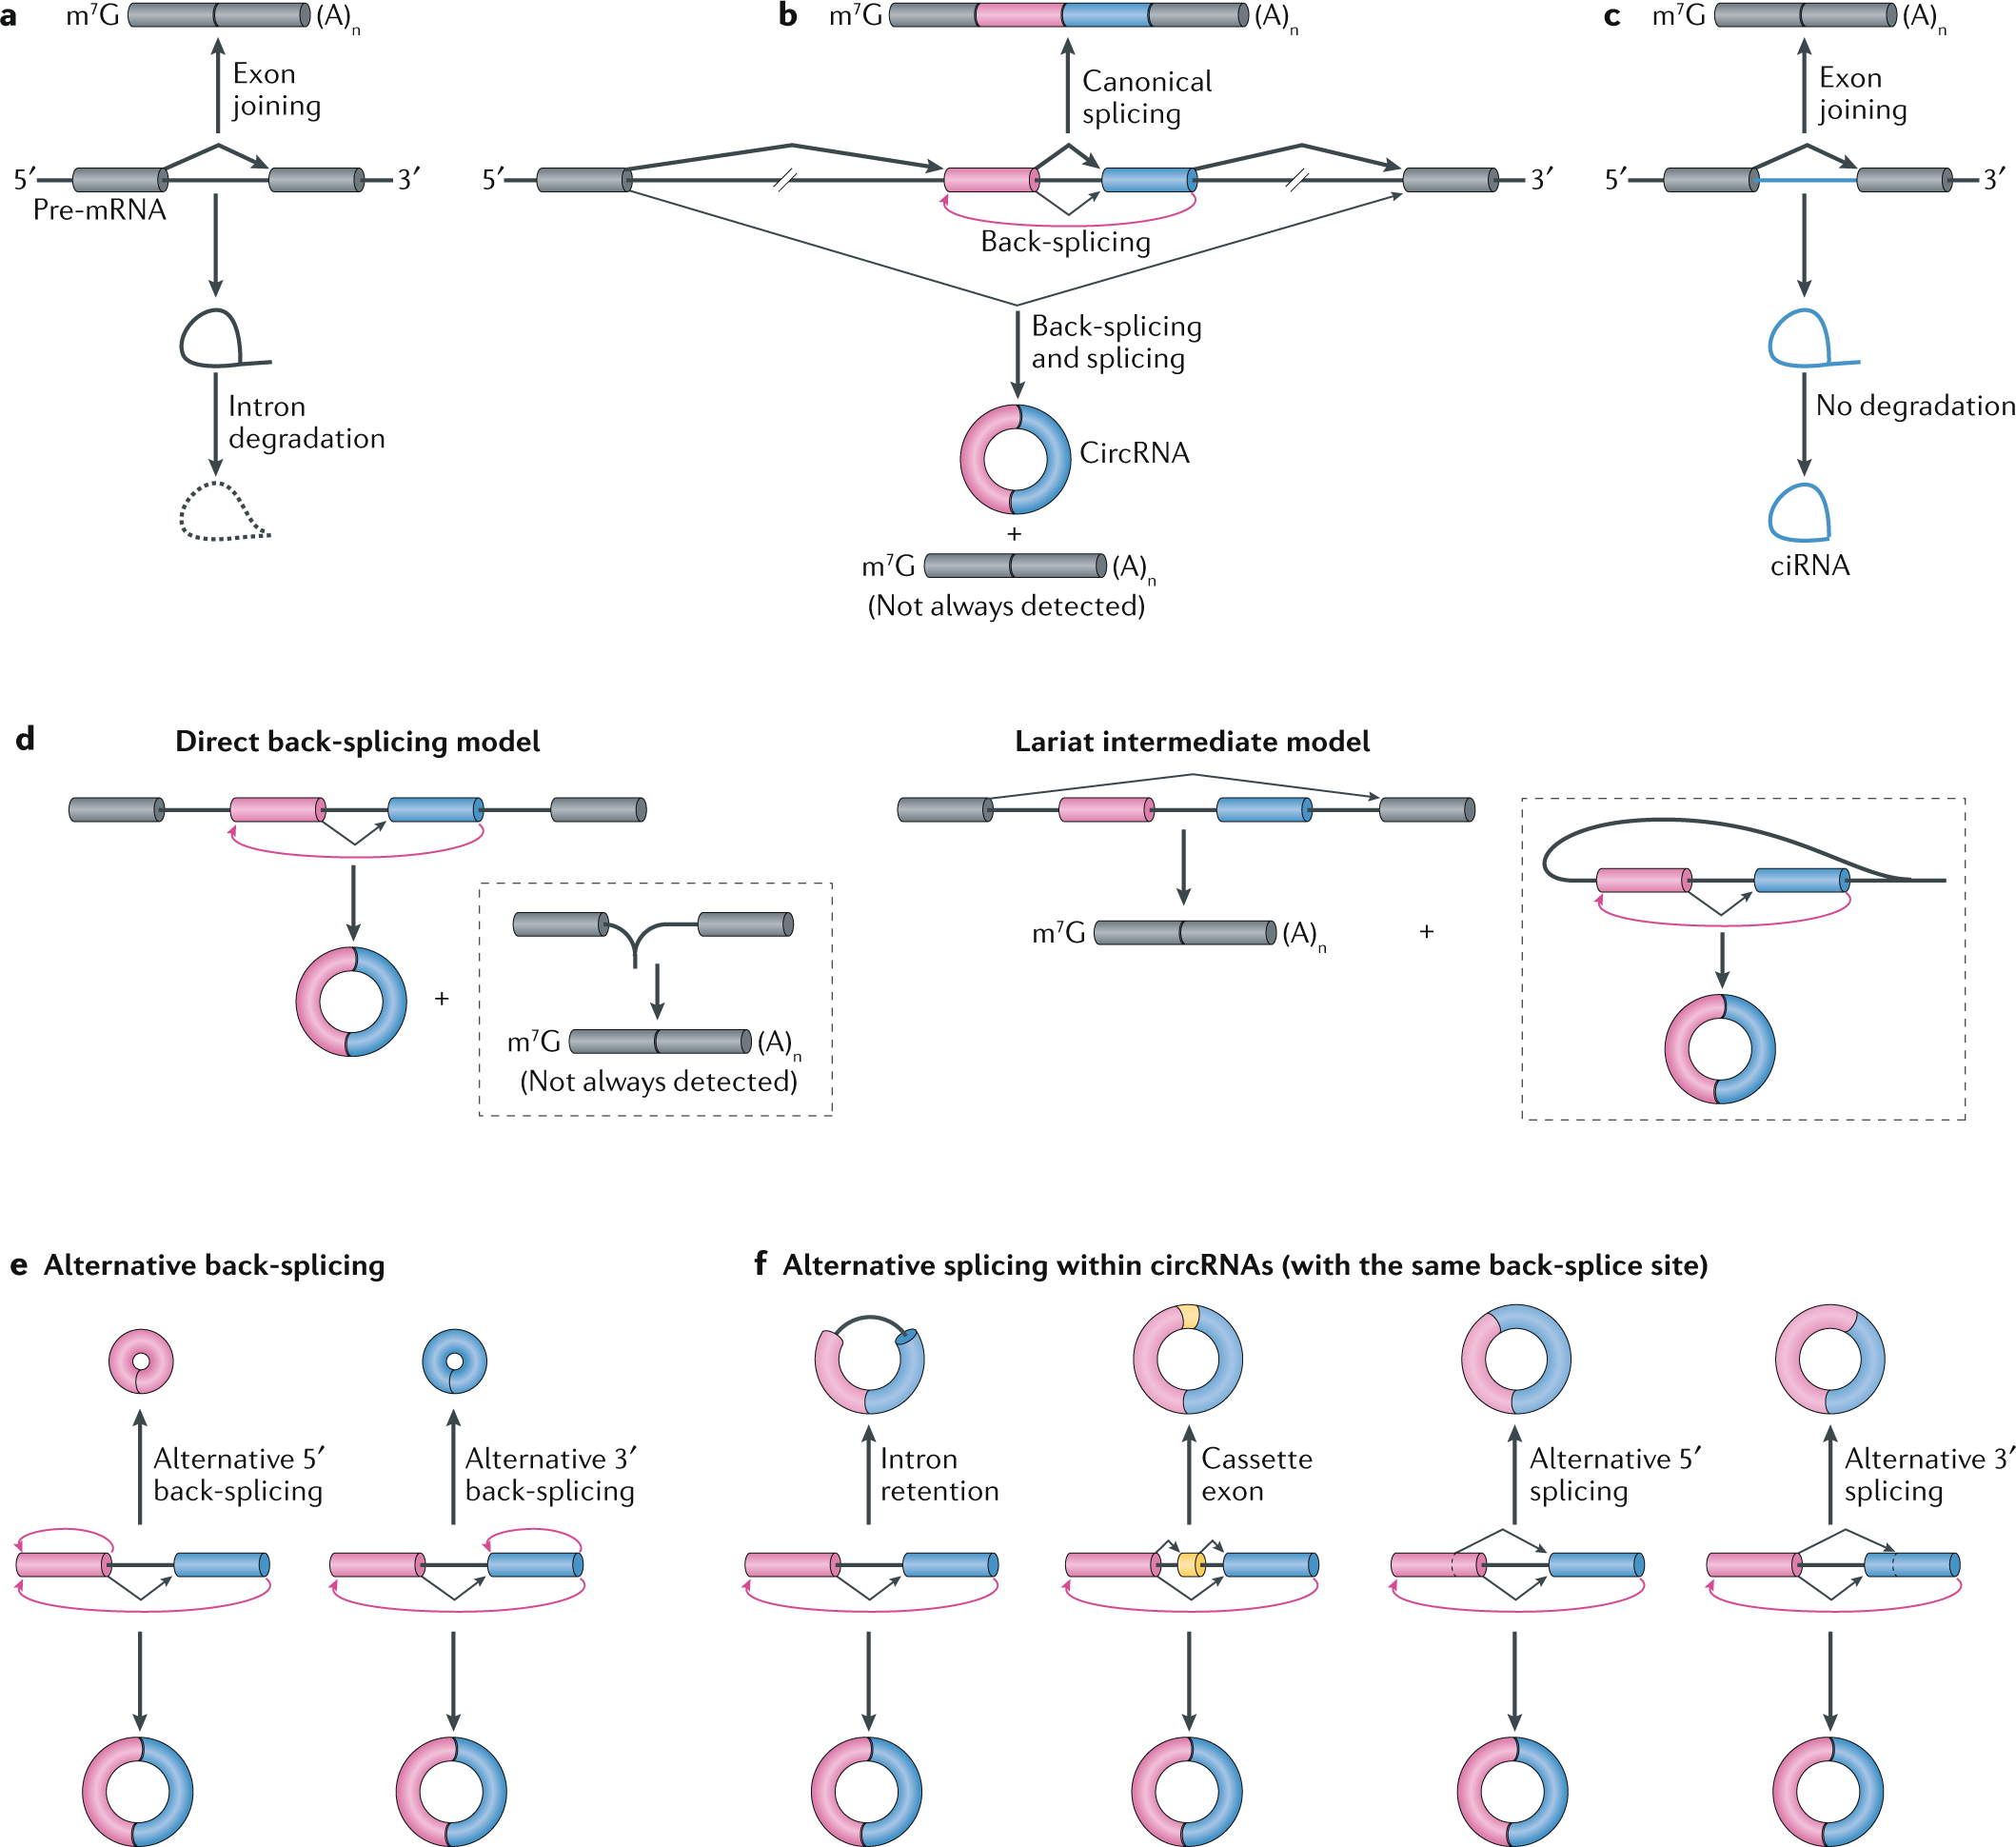
\includegraphics[width=\textwidth]{chapters/background/figures/circRNA-splicing.png}
    \caption{Splicing of circRNAs} % TODO: Add detailed caption
    \label{fig:circRNA_splicing}
\end{figure}

\subsection{circRNA types}
\iffalse
\subsubsection{Circular intronic RNAs (ciRNAs)}
Introns typically form a lariat shape during conventional splicing, which is
generally debranched and degraded soon after splicing
(\cref{fig:circRNA_splicing}a). However, in some cases, introns evade
debranching and instead form covalently bonded circular RNA molecules
(\cref{fig:circRNA_splicing}c), known as circular intronic RNAs (ciRNAs)
\supercite{chen_expanding_2020,zhang_circular_2013}.

\subsubsection{Exonic circular RNAs (EcircRNAs)}
EcircRNAs are generated from exon-skipping events. Here, the lariat contains at
least one exon and potentially multiple introns. The introns are subsequently
removed through internal splicing, producing a circular RNA molecule composed
solely of exonic sequences \supercite{xiao_circular_2022, li_biogenesis_2018}.

\subsubsection{Exon-intron circular RNAs (EIcircRNAs)}
The formation of EIcircRNAs is similar to that of EcircRNAs, with the exception
that introns are not completely removed during splicing, resulting in a circular
RNA molecule containing both exonic and intronic sequences
\supercite{xiao_circular_2022}.
\fi

\paragraph{Exonic circular RNAs (ecircRNAs)} are the most prevalent type of
circRNAs, primarily formed from back-splicing of exons from protein-coding genes. They are
typically located in the cytoplasm and can function as sponges for microRNAs
(miRNAs), thereby modulating gene expression and influencing various cellular
processes, including tumorigenesis and cellular differentiation (Bachmayr-Heyda
et al., 2015; Wang et al., 2021). EcircRNAs have been shown to interact with
RNA-binding proteins, which can further regulate their stability and function
(Zang et al., 2018). Their abundance and stability make them potential
biomarkers for various diseases, including cancers (Li et al., 2021; Wang et
al., 2021).

\paragraph{Intronic circular RNAs (ciRNAs)}, on the other hand, are derived from introns
and are predominantly localized in the nucleus. They play a role in regulating
the transcription of their parental genes and are characterized by their
constrained expression patterns (Ma et al., 2020; Xie et al., 2023). ciRNAs are
believed to interact with components of the transcription machinery, thereby
influencing gene expression at the transcriptional level (Reddy et al., 2017).
The nuclear localization of ciRNAs suggests they may have distinct regulatory
functions compared to their ecircRNA counterparts.

\paragraph{Exon-Intron Circular RNAs (EIciRNAs)} are a hybrid form that includes both
exonic and intronic sequences. Like ciRNAs, EIciRNAs are also found in the
nucleus and have been implicated in the regulation of gene transcription. They
can enhance the expression of their parent genes by interacting with RNA
polymerase II and other transcription factors (Chen et al., 2022; Su, 2024).
This dual composition allows EIciRNAs to potentially serve as intermediaries in
the regulation of gene expression, bridging the functions of both ecircRNAs and
ciRNAs.

\paragraph{Intergenic circular RNAs (IcircRNAs)} are formed from regions of the genome
that do not code for proteins and are often less characterized than the other
types. Their functions remain largely unknown, but they are thought to
contribute to the regulatory networks within cells, possibly by interacting with
other RNA molecules or proteins (Li et al., 2021). The study of IcircRNAs is
still in its infancy, and further research is needed to elucidate their roles in
cellular processes.

\subsection{Biological functions}
circRNAs have emerged as key players in various biological processes, showcasing
a wide range of functions that contribute substantially to cellular regulation.

\subsubsection{Micro RNA sponging}
One of the most well-documented functions of circRNAs is their ability to act as
miRNA sponges. This mechanism involves the binding of circRNAs to specific
miRNAs, thereby preventing these miRNAs from interacting with their target
mRNAs. For instance, the circRNA CDR1as has been shown to contain over 60
binding sites for miR-7, effectively sequestering it and allowing the expression
of miR-7 target genes to increase\supercite{guo_expanded_2014,yuan_regulatory_2020}. This
competitive endogenous RNA (ceRNA) activity is crucial in regulating gene
expression and has been implicated in various cancers, including gliomas and
gynecological cancers\supercite{dong_expression_2020,song_circular_2016}. Additionally,
circRNAs such as circ-0000437 have been identified as sponges for miRNAs
involved in tumor progression, highlighting their potential as therapeutic
targets\supercite{li_peptide_2021,cui_circular_2022}.

\subsubsection{Protein interactions}
Beyond miRNA sponging, circRNAs also participate in protein interactions. They
can serve as scaffolds for RNA-binding proteins (RBPs), influencing various
cellular processes, including transcription and
splicing\supercite{li_comprehensive_2017,qu_emerging_2017}. For example,
circRNAs can recruit RBPs to specific genomic loci,
thereby modulating the transcriptional landscape of the cell\supercite{li_comprehensive_2017}.
This interaction can lead to the regulation of gene expression at multiple
levels, further emphasizing the multifaceted roles of circRNAs in cellular
biology\supercite{zhang_important_2024,he_targeting_2021}. Moreover, some circRNAs have been shown
to interact with proteins that are involved in signaling pathways, such as the
Wnt/\textbeta{}-catenin pathway, thereby influencing cellular proliferation and
differentiation\supercite{peng_novel_2021}.

\subsubsection{Translation into peptides}
In the canonical initiation of translation, ribosomes bind to the 5' cap of an
mRNA \supercite{hinnebusch_mechanism_2012}. Because circRNAs are circular and
lack a 5' cap, they were long thought to be non-coding
\supercite{bao_regulatory_2019,greene_circular_2017}. However, research has
shown that circRNAs with internal ribosome entry sites can indeed be translated
into proteins \supercite{chen_expanding_2020}:

\paragraph{Internal ribosome entry sites (IRES)}
In 1988, researchers discovered that certain viral and cellular mRNAs contain
sequences allowing ribosomes to initiate translation without a 5' cap
\supercite{pelletier_internal_1988, jang_segment_1988}. These sequences are
known as internal ribosome entry sites (IRES). In 1995, Chen and Sarnow
demonstrated that artificially engineered circRNAs containing an IRES sequence
are translated into peptides \supercite{chen_initiation_1995}. Later, it
was found that some circRNAs naturally possess IRES sequences and can thus be
translated into peptides
\supercite{chen_expanding_2020,legnini_circ-znf609_2017,pamudurti_translation_2017}.
A concrete example for an IRES is the consensus motif for
N\textsuperscript{6}-methyladenosine modification \supercite{yang_extensive_2017}.

\paragraph{N\textsuperscript{6}-methyladenosine (m\textsuperscript{6}A)}
% General introduction to m6A
m\textsuperscript{6}A is the most abundant base modification in eukaryotic RNA
\supercite{yang_extensive_2017,li_pivotal_2014,wei_methylated_1975}. Research
has shown that m\textsuperscript{6}A modification can affect localization,
splicing, translation and degradation of RNA molecules
\supercite{yue_rna_2015,meyer_dynamic_2014}. The effect of m\textsuperscript{6}A
modification on translation is particularly interesting, as it has been shown
that m\textsuperscript{6}A modifications in 3' UTRs can enhance translation
efficiency\supercite{wang_n6-methyladenosine_2015}, while m\textsuperscript{6}A
modifications in 5' UTRs can promote cap-independent translation, especially in
heat shock stress\supercite{zhou_dynamic_2015,meyer_5_2015}.

% Build bridge to IRES-dependent mechanism
m\textsuperscript{6}A modifications mostly occur in the consensus motif
RRm\textsuperscript{6}ACH (R = purine, H = non-guanine base)
\supercite{csepany_sequence_1990,harper_sequence_1990}, which has been found to
be enriched in circRNAs \supercite{yang_extensive_2017}. In circRNAs, a single
m\textsuperscript{6}A modification is often enough to initiate
translation\supercite{yang_extensive_2017}.

\subsection{Potential applications}
The unique properties of circRNAs, such as their stability, abundance, and
specific expression patterns, make them attractive candidates for various
applications in the field of molecular biology and medicine. Their potential
uses include serving as biomarkers for disease diagnosis and prognosis,
therapeutic targets for drug development, and tools for gene regulation and
editing.

\subsubsection{Biomarkers}
One of the most compelling applications of circRNAs lies in their potential as
biomarkers for cancer diagnosis and prognosis. Studies have demonstrated that
circRNAs can serve as reliable indicators of tumor progression and treatment
response. For instance, circRNAs exhibit higher expression levels in certain
cancers compared to their linear counterparts, suggesting their utility in
liquid biopsies for non-invasive cancer
monitoring\supercite{bao_prognostic_2020,ren_construction_2017}. Their stability
in bodily fluids such as plasma and saliva further
enhances their applicability as biomarkers, as they are less prone to
degradation than traditional RNA
markers\supercite{bao_prognostic_2020,zhang_circular_2018}. Specific circRNAs,
such as hsa\_circ\_0000190, have been correlated with
advanced stages of lung cancer, indicating their potential role in clinical
settings\supercite{luo_plasma_2020}. Moreover, circRNAs have been implicated in
chemoresistance, providing insights into treatment efficacy and patient
management\supercite{geng_function_2018,feng_functions_2019}.

Beyond their role in cancer, circRNAs are also being explored in the context of
autoimmune diseases and neurological disorders. For example, circRNAs have been
identified as novel biomarkers for rheumatoid arthritis and multiple sclerosis,
highlighting their versatility in reflecting disease states beyond
oncology\supercite{ouyang_identification_2021,he_exosomal_2019}. Their
expression profiles in various
tissues suggest that circRNAs may play a role in the pathophysiology of these
conditions, potentially guiding therapeutic strategies\supercite{mohammed_circular_2023}.

\subsubsection{Therapeutic targets}
In addition to their diagnostic potential, circRNAs are being investigated as
therapeutic targets. Their ability to modulate gene expression and interact with
microRNAs positions them as key regulators in cellular processes, including
those involved in cancer stem cell dynamics and immune
responses\supercite{cheng_emerging_2023}. Emerging research indicates that
circRNAs can be engineered for
therapeutic purposes, such as enhancing the efficacy of RNA-based therapies like
CRISPR and siRNA\supercite{wesselhoeft_engineering_2018}. This opens avenues for innovative
treatment strategies that leverage the unique properties of circRNAs to combat
diseases more effectively.